\documentclass[a4paper,10pt]{article}
\usepackage[utf8]{inputenc}
\usepackage{amsmath}
\usepackage{graphicx}
\numberwithin{equation}{section}
%opening
\title{Math Phys II HW 2}
\author{Vince Baker}

%opening
\title{}
\author{Vince Baker}

\begin{document}

\maketitle

\begin{abstract}

\end{abstract}

\section{Problem 1}
We solve the harmonic oscillator by writing down the classical Hamiltonian, replacing the momentum by $\frac{\hbar}{i}\frac{d}{dx}$, and solving.
The classical Hamiltonian is:
\begin{equation}
H=\frac{p^2}{2m}+\frac{1}{2}kx^2
\end{equation}
Replacing p with $\frac{\hbar}{i}\frac{d}{dx}$:
\begin{gather}
\{ \frac{-\hbar ^2}{2m}\frac{d^2}{dx ^2}+\frac{1}{2}kx^2\}\Psi=E\Psi\\
\frac{d^2 \Psi}{dx^2}-\frac{mkx^2}{\hbar ^2}\Psi+\frac{2mE}{\hbar^2}\Psi=0
\end{gather}
We now make a transformation $x=\gamma z$ into dimensionaless coordinates.
\begin{gather}
\frac{1}{\gamma ^2}\frac{d^2 \Psi}{dz^2}-\frac{mk}{\hbar ^2}\gamma^2z^2\Psi+\frac{2mE}{\hbar^2}\Psi=0\\ 
\frac{d^2 \Psi}{dz^2}-\frac{mk}{\hbar ^2}\gamma^4z^2\Psi+\frac{2mE}{\hbar^2}\Psi=0\\ 
\end{gather}
Table 22.6 of A\&S has the solution for this general form, with the coefficient of the z term $2n+1-x^2$.
The solutions are $e^{\frac{-x^2}{2}}H_n(x)$ with $H_n(x)$ the Hermite polynomials. 
Solving for the dimensionless parameter $\gamma$ we find:
\begin{gather}
\frac{mk}{\hbar ^2} \gamma ^4=1\\
\gamma ^2=\frac{\hbar }{\sqrt{mk}}\\
\frac{2mE}{\hbar ^2}\gamma ^2=2n+1\\
E=\frac{\hbar ^2}{2m}\frac{\sqrt{mk}}{\hbar}(2n+1)=\hbar \sqrt{\frac{k}{m}}(n+\frac{1}{2})
\end{gather}
We plot the analytic solutions for the 1-D quantum harmonic oscillator. 
\begin{equation}
 \Psi(x)_n=\frac{1}{\sqrt{2^n n! \sqrt{\pi}}}H_n(x)
\end{equation}
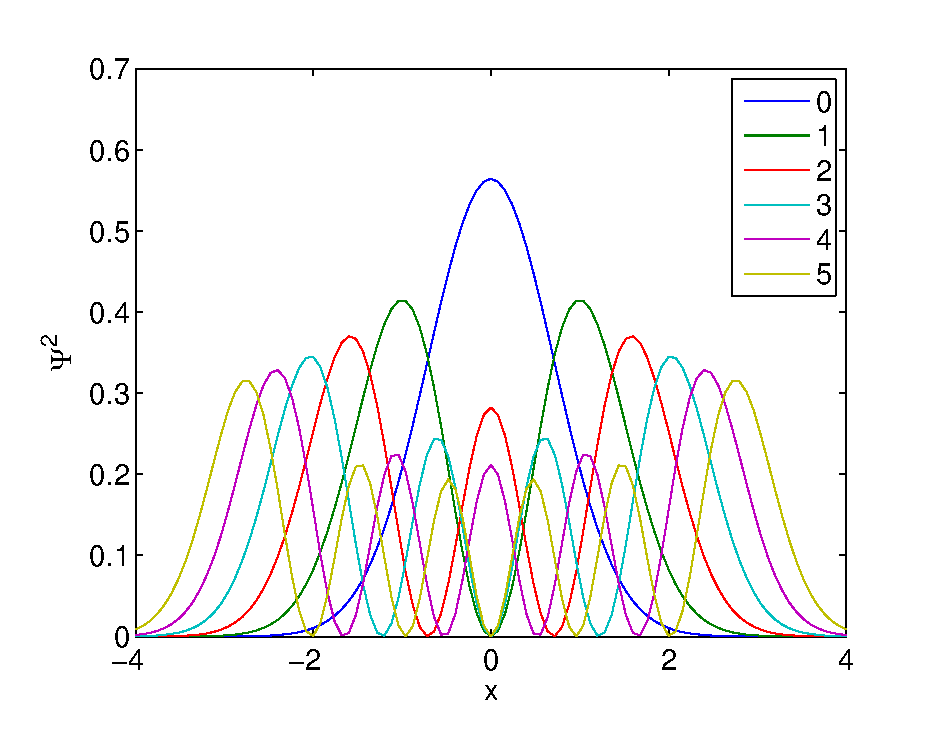
\includegraphics{analytic}
\section{Problem 2}
We now solve the quantum harmonic oscillator using a numerical method.
We'll set $\hbar =k=m=1$ to simplify the expressions.
We approximate the second derivative as:
\begin{equation}
\frac{d^2}{dx^2}=\frac{x_{i+1}-2x_{i}+x_{i-1}}{\Delta ^2} 
\end{equation}
As a matrix operator this can be written:
\begin{equation}
\begin{pmatrix}
-2 & 1 & 0 & \cdots & 0\\
1 & -2 & 1 & \cdots & 0 \\
\vdots & \ddots & \ddots & \ddots & \vdots\\
0 & 0 & \cdots & 1 & -2
\end{pmatrix}
\end{equation}
The potential energy is simply the diagonal matrix with $x_i^2$'s on the diagonal, multiplied by $\frac{1}{2}$.
We can now write the Schrodinger equation in a matrix form:
\begin{equation}
(K_e+P_e)\Psi=E\Psi 
\end{equation}
With $\Psi$ a column vector. This is clearly in the form of an eigenvalue problem, which we solve using MATLAB. 
The 6 lowest eigenvalues are (to within .01) 0.5, 1.5, 2.5, 3.5, 4.5 and 5.5 in close agreement with the analytical energy levels $n+\frac{1}{2}$ (ignoring the scaling factor). 
Increasing the number of lattice sites from 101 to 1001 improves the agreement to .001.
We plot the eigenvectors corresponding to the 6 lowest eigenvalues.
\linebreak

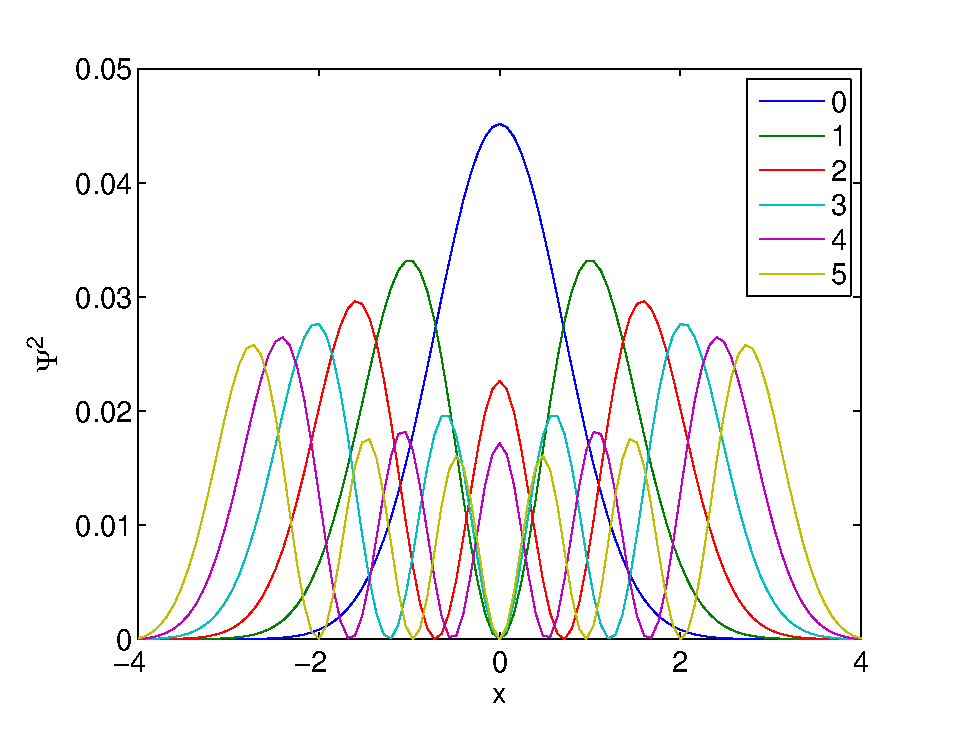
\includegraphics{numeric1}

\section{Problem 3}
We now solve the harmonic oscillator using a variational principle on the quadratic form of the Schrodinger equation.
Again setting $\hbar =k=m=1$, we have:
\begin{equation}
J=\int (\frac{d\Psi }{dx})^{2}+\frac{1}{2}kx^2\Psi ^2 dx\\
\end{equation}
We apply a normalization constraint to avoid the trivial solution $\Psi=0$, and incorporate the constraint via Lagrange multipler.
\begin{gather}
\int \Psi^2 dx = 1\\
J=\int (\frac{d\Psi }{dx})^{2}+\frac{1}{2}kx^2\Psi ^2 dx - E\int \Psi^2 dx
\end{gather}
We decompose $\Psi$ into a sum of localized basis functions $\Psi_i=c_ie^{\frac{-(x-x_i)^2}{2\sigma ^2}}$.
We now need to calculate the integrals of $(\frac{d\Psi }{dx})^{2}$, $x^2\Psi ^2$, and $\Psi^2$.
We write $\Psi^2$ in this basis as:
\begin{gather}
 \sum_{i}\sum_{j}c_ic_je^{\frac{-(x-x_i)^2}{2\sigma ^2}}e^{\frac{-(x-x_j)^2}{2\sigma ^2}}\\
 \sum_{i}\sum_{j}c_ic_je^{\frac{-(x-x_i)^2-(x-x_j)^2}{\sigma ^2}}
\end{gather}
Pulling the coefficients outside, and letting $\sigma=\Delta x$, this integral (according to Wolfram Alpha) is:
\begin{gather}
\frac{\sqrt{\pi}}{2}\sigma e^{\frac{-(i-j)^2}{4}}\{erf(\frac{x_i+x_j+8}{2\sigma})-erf(\frac{x_i+x_j-8}{2\sigma})\}
\end{gather}
For reasonably small values of $\sigma$ the error function becomes a step function at 0, and the right hand term becomes 2 for all values of i and j.
The  exponential will suppress all terms where $|i-j|$ is not small. We cut off all terms with  $|i-j|<6$, so the next term is less then $\frac{1}{1000}$.
\begin{gather}
 \sum_{i}\sum_{j=i-5}^{i+5}c_ic_j\sqrt{\pi}\sigma e^{\frac{-(i-j)^2}{4}}
\end{gather}
For the potential term we need to caclulate the integral of $x^2\Psi ^2$. 
This integral is not calculated by Wolfram Alpha, so we use the solution provided in class.
\begin{gather}
 \sum_{i}\sum_{j=i-5}^{i+5}c_ic_j\sqrt{\pi}\sigma e^{\frac{-(i-j)^2}{4}}(\frac{x_i+x_j}{2}^2+\frac{1}{2}\sigma ^2)
\end{gather}
We find the derivative of $\Psi$ anaylytically, then calculate the integral of $(\nabla \Psi)^2$ using the previous integrals.
\begin{gather}
\nabla \Psi= \sum_{i}c_i\frac{d}{dx}e^{\frac{(x-x_i)^2}{2\sigma ^2}}\\
\nabla \Psi=\sum_{i}c_i\frac{-(x-x_i)}{\sigma ^2}e^{\frac{(x-x_i)^2}{2\sigma ^2}}\\
\int (\nabla \Psi)^2 = \int \sum_{i}\sum_{j}c_ic_j\frac{x-x_i}{\sigma ^2}\frac{x-x_j}{\sigma ^2}
  e^{\frac{(x-x_i)^2}{2\sigma ^2}}e^{\frac{(x-x_j)^2}{2\sigma ^2}}\\
  =\sum_{i}\sum_{j}\frac{\sqrt{\pi}}{\sigma}e^{\frac{(i-j)^2}{4}}\{(\frac{x_i+x_j}{2})^2+\frac{1}{2}\sigma ^2
  -(x_i+x_j)\frac{x_i+x_j}{2}
  +x_ix_j\}c_ic_j\\
  =\sum_{i}\sum_{j}\frac{\sqrt{\pi}}{\sigma}e^{\frac{(i-j)^2}{4}}\{-\frac{(x_i+x_j)^2}{4}+\frac{1}{2}\sigma ^2+x_ix_j\}c_ic_j\\
  =\sum_{i}\sum_{j=i-5}^{i+5}\frac{\sqrt{\pi}}{\sigma}e^{\frac{(i-j)^2}{4}}\{-\frac{(x_i+x_j)^2}{4}+\frac{1}{2}\sigma ^2+x_ix_j\}c_ic_j
\end{gather}
Where we again only evaluate integrals for  $|i-j|<6$.
We can now make a quadratic form from 3.7, 3.8 and 3.14 in the c's and set up the variational problem in matrix form.
\end{document}
